\chapter{Evaluación Experimental} \label{evaluacion}
En este capítulo se divide en dos secciones, en la primera se describen los experimentos realizados para medir la eficiencia y eficacia de los sistemas implementados. En la segunda parte se muestran los resultados obtenidos.

\section{Dataset y Experimentos}\label{experimentos}
Para probar el sistema se recopiló una colección de videos correspondientes a películas de dominio público. Las peliculas fueron descargadas de un canal de Youtube que se especializa en subir recolectar y subir películas de dominio público\footnote{https://www.youtube.com/user/BestPDMovies}. En total se descargaron 119 películas que corresponden a alrededor de 110 horas de video. El dataset contiene películas publicadas desde 1920 y hasta la década de 1970 cuya protección de derechos de autor expiró, además de algunas más recientes que renunciaron a tales derechos. Debido a esto el dataset presenta videos con un amplio rango de tamaños y calidad de video, además de contener tanto filmes a color como en blanco y negro. 

Para comparar la eficacia de los distintos descriptores se usó la versión distribuida de la aplicación. Esto debido que es la que cuenta con el preprocesamiento encargado de ajustar el video a los límites indicados por el usuario, sin esto los descriptores globales no pueden funcionar para videos de tamaño indeterminado, como en la base de datos recopilada.

Para realizar las pruebas se seleccionaron aleatoriamente 10 videos de la base de datos, y para cada uno se realizaron 4 consultas con cada descriptor, esto nos da un total de 120 consultas. Se estudió el comportamiento de los descriptores al variar la cantidad de objetos en la base de datos de referencia. Para aislar el efecto de la cantidad de películas en la base de datos se guardaron, para cada consulta, los descriptores enviados por el cliente, de esta forma al repetir la consulta con una base de datos mayor podemos estar seguro que cualquier cambio en la efectividad fue debido al cambio en la base de datos y no a cambios del descriptor mismo. Se repitieron las consultas variando la cantidad de películas en la base de datos entre 15 y 119. Para cada consulta se midió la proporción de resultados correctos en comparación con la cantidad total de consultas.

Para probar la eficiencia del sistema distribuido en comparación con el centralizado se midió tanto el tiempo de respuesta total del sistema como la cantidad de datos enviada por el cliente. 

El tiempo de respuesta se midió como el intervalo de tiempo desde que el cliente empieza a enviar datos hasta que termina de recibir la respuesta del servidor. Resulta interesante desglosar este tiempo en etapas para saber que operaciones son más costosas para el sistema. Para esto se midió en el servidor el tiempo gastado en distintas operaciones. En el caso del sistema centralizado se midió el tiempo usado por la extracción de descriptores y por la búsqueda en la base de datos. Para el caso del sistema distribuido se midió el tiempo usado escribiendo los archivos necesarios por P-VCD y los descriptores, así como el tiempo de la búsqueda en la base de datos. Finalmente se calculó el tiempo usado transmitiendo datos bajo el supuesto que:
\begin{equation*}
\displaystyle{Tiempo\ total\ de\ respuesta}  =  \displaystyle{Tiempo\ de\ transmisi\acute{o}n} + \displaystyle{Tiempo\ total\ del\ servidor} 
\end{equation*}

\section{Resultados}\label{resultados}
A continuación se presentan los resultados de los experimentos realizados y su interpretación. 

\subsection{Eficacia}

La figura~\ref{resultados_precision} muestra los resultados de medir la precisión del sistema, esto es, la proporción de resultados correctos con respecto al total de consultas. Podemos apreciar en la figura que  solo uno de los descriptores obtuvo resultados favorables. El descriptor KFD alcanzó una precisión cercana al 56\% en los experimentos realizados, mientras que los otros no superaron en ningún caso el 5\%. Todos los descriptores mostraron una disminución en su precisión al aumentar el tamaño de la base de datos.

	\begin{figure}[!h]
		\centering
		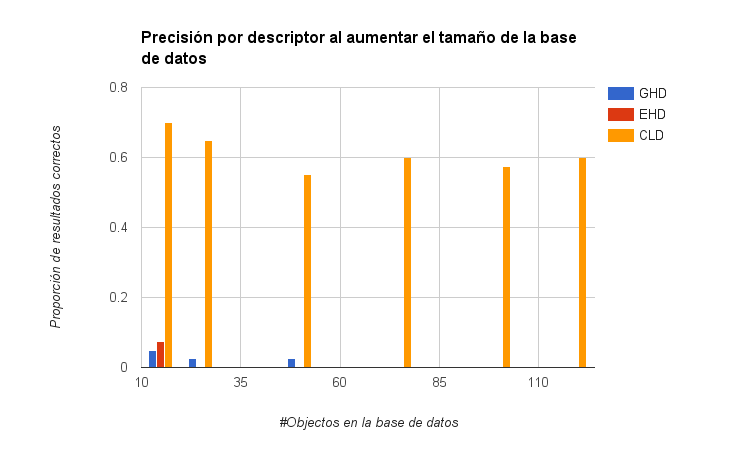
\includegraphics[width=\textwidth]{imagenes/cap5/resultados_precision.png}
		\caption{Gráfico con los resultados de medir la precisión cada descriptor}
		\label{resultados_precision}
	\end{figure}

Para explicar la diferencia en el desempeño de los descriptores debemos fijarnos en la manera en que cada uno extrae características de la imagen y en como los afecta la distorsión provocada por grabar una pantalla con le celular. Un efecto importante que desfavorece al descriptor GHD es que al encuadrar incorrectamente el video se puede grabar accidentalmente parte del marco de la televisión por lo que al calcular el histograma se contarán pixeles que no existen en el video original, más aún, el marco de una televisión típicamente es de un solo color, por lo que todos los pixeles extra se concentrarán en unos pocos bins, provocando en ellos un cambio significativo. Este cambio provoca un mayor efecto en el descriptor que cambiar levemente muchos bins dado que se comparan usando distancia euclideana. En contraste en el caso del KFD el mismo error (grabar pixeles que no existen en el video original) se suavizará debido a que se calculan promedios de pixeles por cada zona. En este caso además el efecto se distribuye sobre todas las zonas afectadas, a diferencia del GHD donde se concentra en unos pocos bins. 
En el caso del descriptor EHD, el efecto que provoca mayor error es probablemente la perdida de calidad de la imagen. Dado que el descriptor se basa en la detección de bordes cambios de calidad que difuminen la imagen hacen que sea más difícil detectar bordes y por ende que este descriptor pierda efectividad. En comparación nuevamente el descriptor KFD se muestra más resistente a tales cambios, pues solo toma en cuenta el valor promedio de los pixeles dentro de un área y no los detalles dentro de la misma.

El buen desempeño del descriptor KFD puede también deberse al dataset utilizado para las pruebas. La base de datos contiene muchas películas en blanco y negro, por lo que al usar el descriptor KFD (que usa el color de la imagen) todas las películas en blanco negro se encontrarán agrupadas en la base de datos, mientras que las películas a color estarán distribuidas de manera más dispersa, facilitando su identificación y mejorando en promedio la precisión del descriptor. Este efecto debería favorecer a cualquier descriptor que haga uso del color de la imagen.

\subsection{Eficiencia}

La figura~\ref{resultados_tiempos_total} muestra la medición del tiempo total de respuesta de cada implementación del sistema y para cada descriptor. De la figura podemos apreciar que para todos los casos la implementación distribuida requiere un tercio menos tiempo en comparación con la implementación centralizada. 

	\begin{figure}[!h]
		\centering
		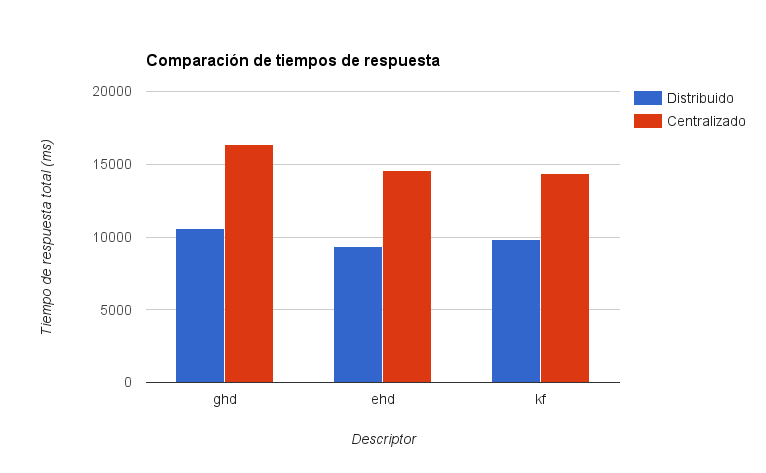
\includegraphics[width=\textwidth]{imagenes/cap5/resultados_tiempos_total.png}
		\caption{Gráfico con comparación de tiempos de respuesta de ambos sistemas}
		\label{resultados_tiempos_total}
	\end{figure}

	\begin{figure}[!h]
		\centering
		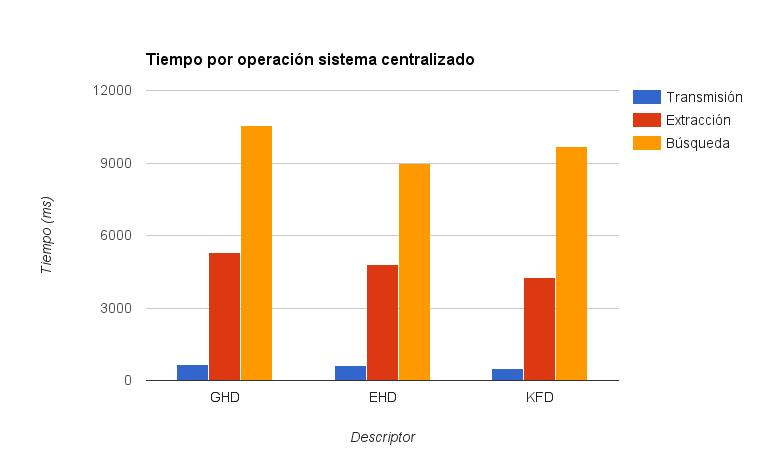
\includegraphics[width=\textwidth]{imagenes/cap5/resultados_tiempo_detalle_centralizado.png}
		\caption{Gráfico con detalle de tiempo por operación del sistema centralizado}
		\label{resultados_tiempo_detalle_centralizado}
	\end{figure}
	
	\begin{figure}[!h]
		\centering
		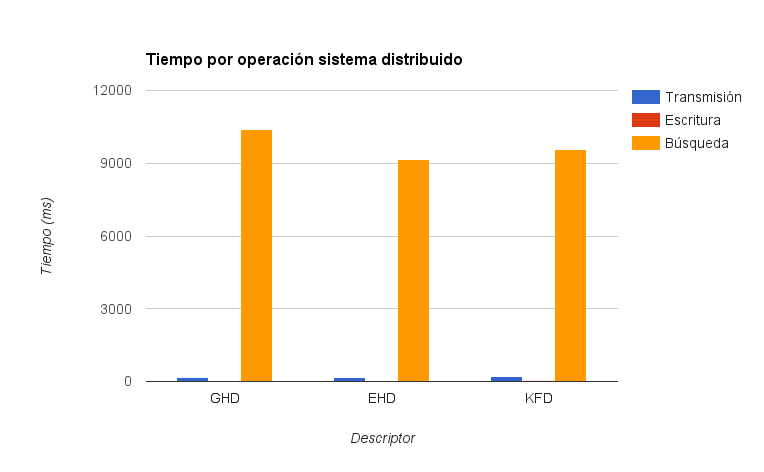
\includegraphics[width=\textwidth]{imagenes/cap5/resultados_tiempo_detalle_distribuido.png}
		\caption{Gráfico con detalle de tiempo por operación del sistema centralizado}
		\label{resultados_tiempo_detalle_distribuido}
	\end{figure}
	
Esta reducción del tiempo de respuesta era de esperarse puesto que la implementación distribuida extrae descriptores mientras el video se graba, presentando un sobrecosto nulo. Para observar de manera más detallada las razones de la disminución del tiempo de respuesta se midió el tiempo requerido por operación. La figuras \ref{resultados_tiempo_detalle_centralizado} y \ref{resultados_tiempo_detalle_distribuido} muestran el detalle del tiempo de cada sistema. Podemos apreciar que en el caso centralizado cerca de un tercio del tiempo total del servidor es usado calculando los descriptores del video de búsqueda. En la versión distribuida este cálculo es reemplazado por simplemente escribir los descriptores recibidos a un archivo, lo cual toma una cantidad despreciable de tiempo en comparación con las otras operaciones. Por otro lado podemos apreciar la disminución del tiempo de transmisión debido a la reducción de la cantidad de datos que hay que enviar al servidor.

Las figuras \ref{resultados_tiempo_detalle_centralizado} y \ref{resultados_tiempo_detalle_distribuido} muestran que para ambas versiones de la aplicación la operación de búsqueda en la base de datos es la más cara en términos de tiempo de procesamiento. Por esto es interesante comprender el comportamiento del tiempo de búsqueda en la base de datos, en particular como varía al crecer el tamaño de la base de datos. La figura \ref{resultados_tiempo_dbquery} muestra los resultados de medir el tiempo usado en la búsqueda al variar el tamaño de la base de datos. El tiempo varía al usar distintos descriptores pues cada uno tiene largo distinto, a más largo el descriptor más tiempo requiere la búsqueda. Del gráfico podemos deducir que el tiempo de búsqueda aumenta linealmente con el tamaño de la base de datos. 

	\begin{figure}[!h]
		\centering
		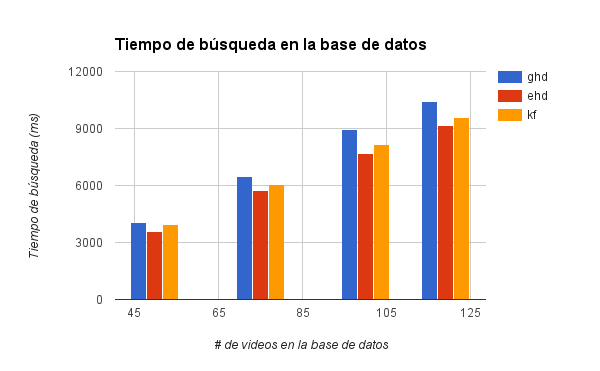
\includegraphics[width=\textwidth]{imagenes/cap5/resultados_tiempo_dbquery.png}
		\caption{Gráfico con tiempos de consulta por descriptor al variar el tamaño de la base de datos}
		\label{resultados_tiempo_dbquery}
	\end{figure}

Finalmente analizamos la cantidad de datos enviados al servidor por cada versión del sistema. La tabla~\ref{resultados_datos_enviados} muestra la comparación de los datos enviados por cada versión. Para la versión distribuida se detalla la diferencia entre cada descriptor. Para la versión centralizada no es necesario el detalle pues no hay diferencia en el video enviado al usar distintos descriptores. Podemos apreciar que se redujo significativamente la cantidad de datos enviados al servidor. La alternativa centralizada envía más de 6 megabytes por cada consulta, mientras que el sistema distribuido reduce esta cantidad al orden de 20 kilobytes dependiendo del tipo de descriptor utilizado. En términos prácticos esta reducción hace posible el usar la aplicación con la red de datos móviles sin incurrir en un gasto excesivo del usuario.

\begin{table}[h]
\centering
\begin{tabular}{|c|c|c|c|l|}
\hline
                                                             & Centralizado & Distribuido - GHD & Distribuido - EHD & Distribuido - KFD          \\ \hline
\begin{tabular}[c]{@{}c@{}}KiloBytes\\ Enviados\end{tabular} & 6389.64      & 22.69             & 11.98             & \multicolumn{1}{c|}{19.60} \\ \hline
\end{tabular}
\caption{Cantidad de datos enviados al servidor por cada versión de la aplicación}
\label{resultados_datos_enviados}
\end{table}